\subsection{Read thermistor values with ADC}
The ADC is a component of the SCA that is used to convert the analog signal of
the thermistors to a digital signal that can be read by the computer.
The readout is a \emph{voltage} ranging from 0 to 1 V.

To measure the voltage across any thermistor connected to the ADC, first the
current source must be switched on for that channel, and then a read command
must be issued.

To perform a readout, first follow \autoref{fig:adc-current-channel} to enable
current source of the channels to readout,
then follow \autoref{fig:adc-readout} to readout a voltage of that channel.

\begin{figure}[ht]
    \centering
    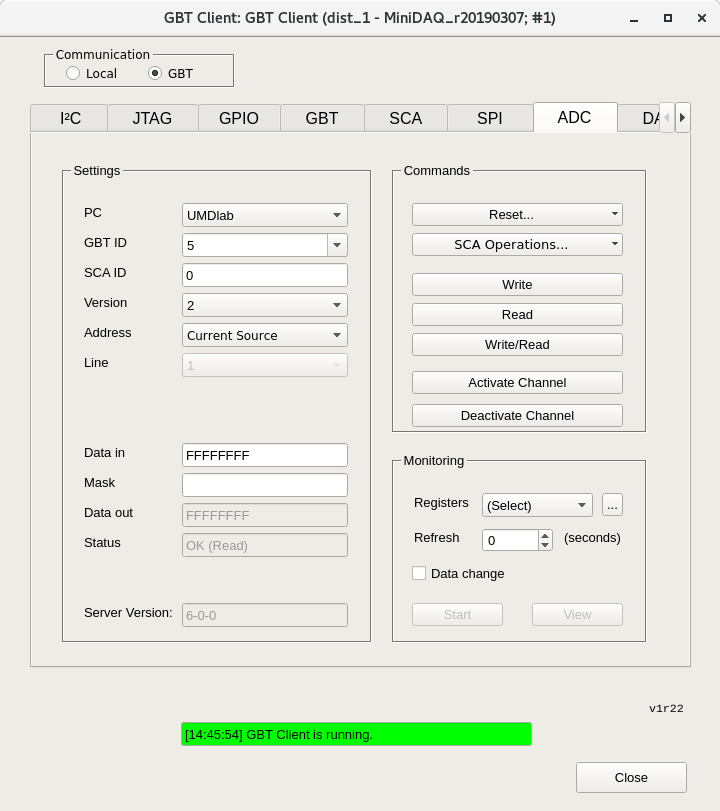
\includegraphics[width=0.9\textwidth]{res/gbt_client_adc_readout_currentsource.png}
    \caption{
        Parameters to send a command to the SCA to activate 100 $\mu$A current
        sources for specific channels.
        For SCAv2, it is OK to enable current source on every channel (thus the
        \texttt{0xFFFFFFFF} in \textbf{Current Source} setting).
    }
    \label{fig:adc-current-channel}
\end{figure}

\begin{table}[ht]
    \begin{tabular}{cccc}
        \toprule
        ADC channel & Signal name & Line & Register setting \\
        \midrule
        \texttt{CH 00} & \texttt{DC\_PLAT\_RTD\_A}    & 0  & Always on \\
        \texttt{CH 01} & \texttt{OM45\_THERM\_Leg\_A} & 1  & \texttt{0x02000000} \\
        \texttt{CH 16} & \texttt{OM23\_THERM\_Leg\_A} & 16 & \texttt{0x00000100} \\
        \texttt{CH 17} & \texttt{OM61\_THERM\_Leg\_A} & 17 & \texttt{0x00000200} \\
        \texttt{CH 18} & \texttt{OMMC\_THERM\_Leg\_A} & 18 & \texttt{0x00000400} \\
        \texttt{CH 31} & Internal SCA thermistor      & ?  & ? \\
        \bottomrule
    \end{tabular}
    \caption{
        Correspondence between control register bits and the channels they
        control.
    }
    \label{tab:register-channel-correspondence}
\end{table}

\begin{figure}[ht]
    \centering
    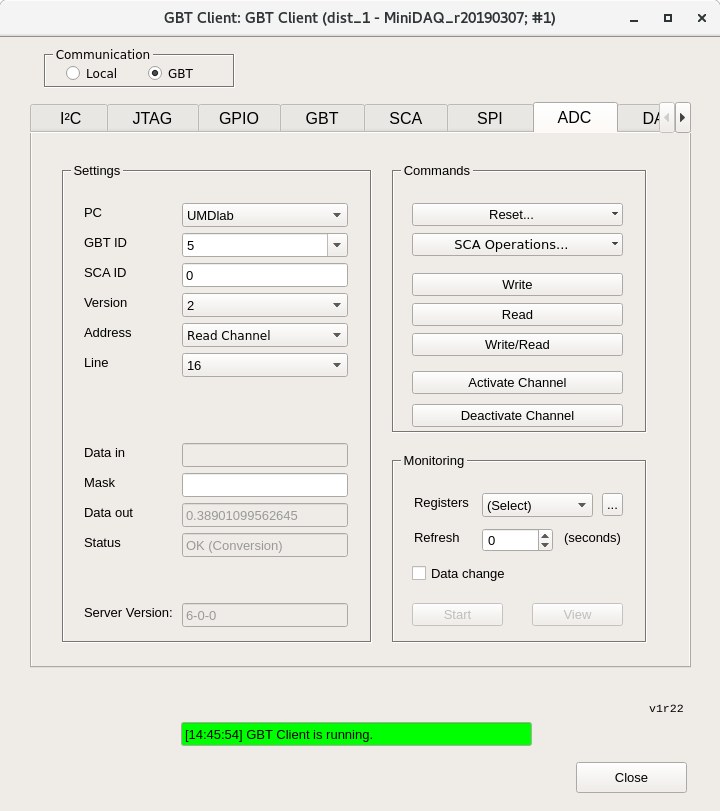
\includegraphics[width=0.9\textwidth]{res/gbt_client_adc_readout_readchannel.png}
    \caption{
        Parameters to send a command to the SCA to read the voltage on the
        channel specified by the given line.
    }
    \label{fig:adc-readout}
\end{figure}

It is important to note that we \emph{should} only enable current source for the
channels that are about to be read.
The correspondence between register bits and the channel they control are listed
in \autoref{tab:register-channel-correspondence}.
Also, \textbf{Version} must be set to \textbf{2}, \textbf{Address} must be set
to the desired command, and \textbf{Line} must be set to the desired channel to
be probed.

For DCB, there are two types of thermistors A platinum-based thermistor on the
DCB mainboard, and another type on the optical mezzanines.
The resistance-temperature curves are listed in \autoref{sec:rt-dcb}
and \autoref{sec:rt-opt-mezz}, respectively.
